\documentclass{article}
%\VignetteIndexEntry{kdetrees Manual}
%\usepackage{fullpage}
\usepackage{natbib}
\usepackage{bibentry}
\nobibliography*

\title{kdetrees Manual}
\author{Grady Weyenberg}
\newcommand{\ape}{{\tt ape}}


\usepackage{Sweave}
\begin{document}
\maketitle

\section{Introduction}
\label{sec:introduction}

KDETrees is a tool for finding discordant phylogenetic trees. It takes
as input a collection of trees (as a {\tt ape::multiPhylo} object),
and produces a unnormalized density \emph{score} for each tree. High
scores mean the tree is relatively similar to other trees in the
sample, while low scores indicate that the tree in question may be
discordant with the others. Low scoring trees are identified as
putative \emph{outliers}, and their contribution to the score
calculation is removed. The result object contains scores for each
tree, and a list of the putative outlier trees. If you use the program
in your research, please cite our paper:
\begin{quote}
  \bibentry{kdetrees}.
\end{quote}


\section{Using {\tt kdetrees}}
\label{sec:use}
%% The simplest method of using the software is the {\tt
%%   kdetrees.complete} function. This is a convienence function which
%% will do all the steps of the analysis at once: importing trees from
%% file, performing the analysis, and producing output files. Basic use
%% is to simply pass it the filename of a Newick file containing the
%% trees to be analyzed. It will write several result files to the R
%% working directory ({\tt getwd}).

%% The call below assumes there is a file containing newick formatted trees
%% named {\tt trees.tre} in the current working directory. It will write
%% out 4 files: {\tt outliers.tre} a newick file containing only the
%% trees identified as outliers; {\tt results.csv} a csv files with the
%% density estimates; {\tt plot.png} and {\tt hist.png} are diagnostic
%% images. The names of these output files can be customized with futher
%% arguments to {\tt kdetrees.complete}.

%% <<kdetrees.complete,eval=FALSE>>=
%% kdetrees.complete("trees.tre")
%% @ 

%% The {\tt kdetrees.complete} function also accepts any of the
%% parameters accepted by the {\tt kdetrees} function, as described in
%% Sections \ref{sec:running-kdetrees} and \ref{sec:advanced-options}.


\subsection{Importing Trees}
\label{sec:importing-trees}

Trees may be imported using any of the methods provided by the {\tt
  ape} package. (See {\tt ?read.tree} and {\tt ?read.nexus} for
examples.) In the following examples, many functions are a part of the
\ape{} package, and it is recommended that you import it. For
example, to load the example {\tt apicomplexa} dataset, I placed the
Newick tree strings into a file named {\tt apicompexa.tre} file and
ran the commands:
\begin{Schunk}
\begin{Sinput}
> library(ape)
> apicomplexa <- read.tree("apicomplexa.tre")
\end{Sinput}
\end{Schunk}
\emph{NB: The apicomplexa dataset is already included in the
  kdetrees package as example data, you do not need to import it. This
  is purely an example showing how to import your own trees.}

kdetrees also provides the {\tt load.trees} function, which searches
for files by directory and file extension.

\subsection{Running kdetrees}
\label{sec:running-kdetrees}

The simplest way to run {\tt kdetrees} is to call the function of the
same name, with the list of trees as the first argument.
\begin{Schunk}
\begin{Sinput}
> result <- kdetrees(apicomplexa, outgroup="Tt")
> result
\end{Sinput}
\begin{Soutput}
Call: kdetrees(trees = apicomplexa, outgroup = "Tt")
Density estimates:
   Min. 1st Qu.  Median    Mean 3rd Qu.    Max. 
-38.740   5.108   6.107   5.472   6.616   7.199 
Cutoff:  

Outliers detected:
 [1] 472.tre 478.tre 488.tre 505.tre 515.tre 553.tre 578.tre
 [8] 585.tre 588.tre 630.tre 641.tre 645.tre 662.tre 725.tre
[15] 745.tre 750.tre
\end{Soutput}
\end{Schunk}

There are 3 main settings which control the method used in the
analysis: the outlier detection tuning parameter ({\tt k}), the
distance computation method ({\tt distance}), and whether or not to
include branch length information in the distance calculation ({\tt
  topo.only}).  The default options are {\tt distance="geodesic"},
{\tt topo.only=FALSE}, and {\tt k=1.5}.


For example, this call uses topology-based dissimilarity map distance.
\begin{Schunk}
\begin{Sinput}
> kdetrees(apicomplexa, k=1.25, distance="diss", topo.only=TRUE)
\end{Sinput}
\end{Schunk}

\begin{figure}
  \centering
\begin{Schunk}
\begin{Sinput}
> plot(result)
\end{Sinput}
\end{Schunk}
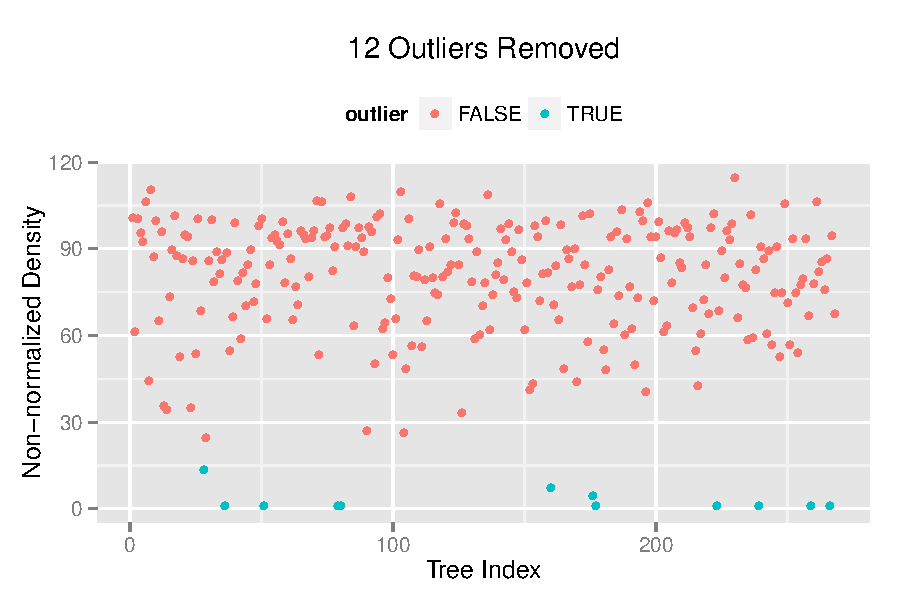
\includegraphics{kdetrees-plot}
\begin{Schunk}
\begin{Sinput}
> hist(result)
\end{Sinput}
\end{Schunk}
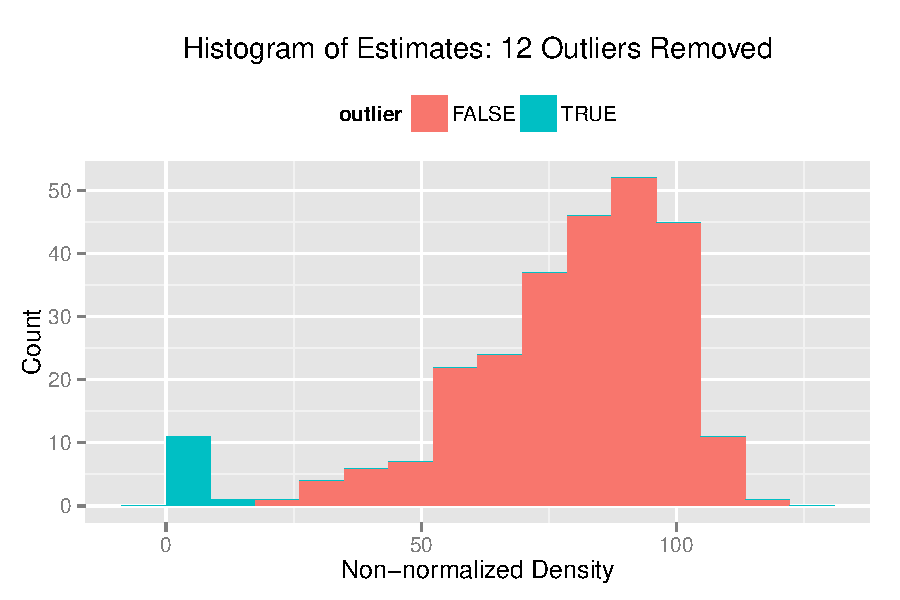
\includegraphics{kdetrees-hist}
  \caption{Diagnostic plots can be created with {\tt plot} and {\tt
      hist}.}
  \label{fig:diagplots}
\end{figure}

One can {\tt plot} or {\tt hist} the result object to create
diagnostic plots. The {\tt plot} and {\tt hist} methods use the
{\tt ggplot2} package, not base graphics, thus you can modify them as
you see fit. See Figure \ref{fig:diagplots} for example plots.

\subsection{Results}
\label{sec:results}

The result object is a list with three components, as well as several
attributes that are used internally.  The first element, {\tt
  density}, has the computed score for each tree in the input
list. This is the variable displayed in the diagnostic plots. The
second element, {\tt i}, contains the indices of the low scoring trees
which were not included in the calculations. Finally, the {\tt
  outliers} element contains the trees which were identified as
outliers.

One might then wish to look at a plot of the putative outlier
trees. Here I plot the lowest scoring tree in the apicomplexa
dataset. It appears that something bad happened during the
reconstruction of this tree, causing one branch to be much longer
than the others.

  \begin{figure}[h]
    \centering
\begin{Schunk}
\begin{Sinput}
> plot(result$outliers[[1]])
\end{Sinput}
\end{Schunk}
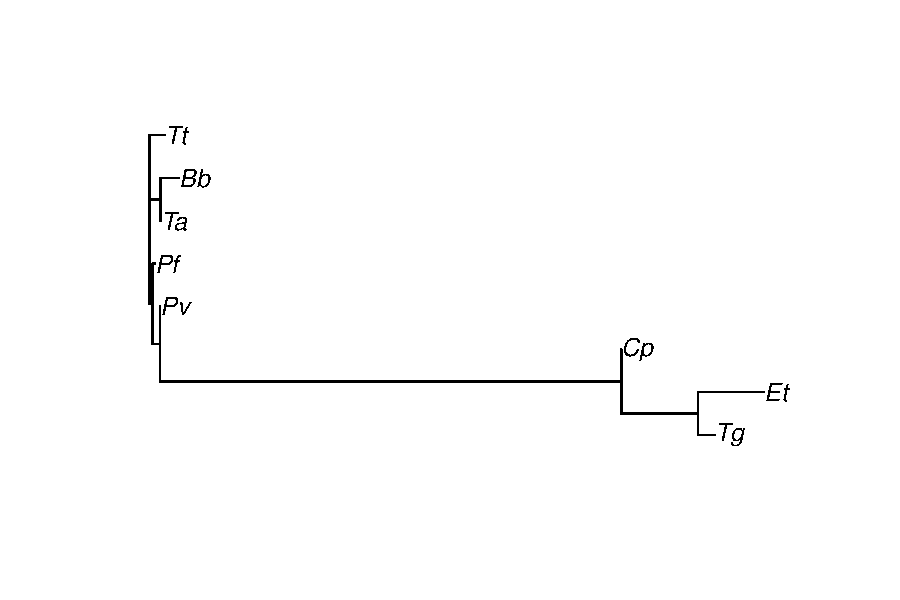
\includegraphics{kdetrees-outlierplot}
    \caption{A plot of an outlying tree.}
    \label{fig:treeplot}
  \end{figure}


  An {\tt as.data.frame} method is provided for the result object,
  which can be used to export the results using the standard R
  methods. (Such as {\tt write.csv}.) The list of outlier trees can be
  exported using {\tt ape::write.tree}
\begin{Schunk}
\begin{Sinput}
> write.tree(result$outliers,file="outliers.tre")
> result.df <- as.data.frame(result)
> write.csv(result.df, file="scores.csv")
\end{Sinput}
\end{Schunk}

\section{Advanced Options}
\label{sec:advanced-options}

\subsection{Distance Methods}
There are currently two methods implemented for the {\tt distance}
option in {\tt kdetrees}: The {\tt "geodesic"} method, based on work
by \citet{bhv}, as well as that of \citet{owen}; and the {\tt "dissimilarity"} map method, which utilizes
pairwise tip-to-top distances.

Each of these distances can use either branch lengths supplied by the
input trees, {\tt topo.only=FALSE}, or the branch lengths can be
ignored by setting {\tt topo.only=TRUE}.


\subsection{Bandwidth Selection}

Currently, kdetrees uses an adaptive bandwidth method based on a
nearest-neighbor calculation by default. It is possible to control the
number of trees used to define the neighborhood, or disable the
adaptive method entirely and provide a constant bandwidth, using the
{\tt bw} parameter. 

If the {\tt bw} parameter is supplied a list, the list is used as a
set of parameters for a call to {\tt bw.nn}. Currently, the only
interesting setting that may be passed in this way is {\tt prop},
which controls the proportion of the set of trees used to define the
neighborhoods. For example, to change the neighborhood to include 50\%
of the sample we pass the following option.
\begin{Schunk}
\begin{Sinput}
> kdetrees(apicomplexa, bw=list(prop=0.5))
\end{Sinput}
\end{Schunk}
If {\tt bw} is set to a single number, a constant bandwidth is used.
\begin{Schunk}
\begin{Sinput}
> kdetrees(apicomplexa, bw=6)
\end{Sinput}
\end{Schunk}
If {\tt bw} is a vector, the values are used as bandwidths for the
corresponding trees in the sample, possibly recycling the values if needed.

\subsection{Command Line Interface}
\label{sec:CLI}

CLI use can be achieved by using the {\tt Rscript} executable included
with R. For example, this CLI command replicates the first example call in
Section \ref{sec:use}.
\begin{verbatim}
$ Rscript -e 'library(kdetrees); kdetrees.complete("trees.tre")'
\end{verbatim}
The desired R commands can also be placed into a R script file
(e.g. {\tt myscript.R}), and run using
\begin{verbatim}
$ Rscript myscript.R
\end{verbatim}

\bibliographystyle{plainnat}
\bibliography{references}


\end{document}
